%! TEX root = main.tex

\graphicspath{{00_Images/10_chapter/}}

\chapter{Horn Loudspeakers}
\label{ch:horns}

The direct-radiating loudspeaker analyzed in the preceding chapters suffers from a fundamental inefficiency: the acoustic impedance of air (\(\rho_0 c \approx \SI{407}{\pascal\second\per\meter}\)) is orders of magnitude lower than the mechanical impedance of the vibrating diaphragm-coil assembly, so the coupling between the mechanical source and the acoustic medium is inherently poor.
The horn addresses this mismatch by acting as an acoustic impedance transformer: a continuously flared duct that progressively increases the acoustic pressure while decreasing the particle velocity, converting the high-impedance motion at its narrow throat into a large-area, low-pressure wave at its wide mouth.
The result is a dramatic increase in radiated acoustic power for a given diaphragm velocity, with efficiencies of 10\% to 50\% routinely achieved compared to the sub-2\% typical of direct radiators.

\section{Principle of Operation and Efficiency}
\label{sc:101}

The operating principle of the horn is a direct application of acoustic impedance transformation.
A diaphragm of area \(S_D\) vibrating at velocity \(u_D\) drives a compression driver whose output throat has a much smaller area \(S_T \ll S_D\).
The horn then expands from throat area \(S_T\) to mouth area \(S_M \gg S_T\), so that the acoustic pressure is amplified by the area ratio and the particle velocity is reduced by the same ratio.
Because power is the product of pressure and volume velocity, this redistribution conserves power while improving the match to the radiation impedance of free air.

\paragraph{Why efficiency is so much higher} In a direct-radiating piston, the radiation resistance \(R_s \propto \omega^2\) is much smaller than \(\rho_0 c\) at low frequencies (\(ka \ll 1\)), meaning that most of the mechanical energy stored in the moving mass and spring is never transferred to the air: it simply circulates as reactive energy between the mechanical elements.
The horn eliminates this mismatch by presenting a high acoustic impedance at the throat, which is where the driver delivers its mechanical power.
The driver therefore sees a largely resistive load at all frequencies above the horn's cutoff, and almost all of its mechanical power is converted into radiated sound.
Typical efficiencies for well-designed horn systems range from 10\% to 50\%, compared to less than 2\% for direct-radiating drivers in the same frequency band.
The theoretical work on horn acoustics was established between 1924 and 1928 in two landmark papers: the first appeared in the Journal of the American Institute of Electrical Engineers in 1924, and the second in the Bell System Technical Journal in 1928.
These papers formalized the horn as an acoustic transformer and introduced the exponential and conical horn profiles that remain the most widely used shapes today.

\begin{figure}[!htb]
    \centering
    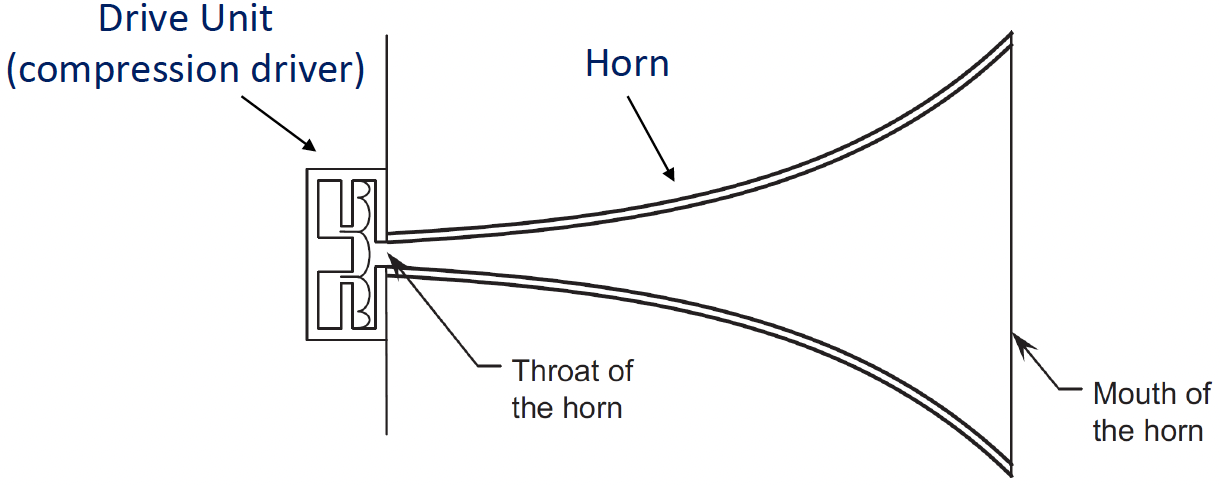
\includegraphics[width=0.70\linewidth]{exp_horn_side.png}
    \caption{Cross-section of a horn loudspeaker with an exponential profile. The compression driver (left) delivers power to the narrow throat of area \(S_T\); the horn expands to the mouth of area \(S_M\), transforming the high-pressure, small-velocity source into a large-area, lower-pressure radiator matched to free air}
    \label{fig:hornSide}
\end{figure}

\section{The Compression Driver}
\label{sc:102}

The transducer element coupled to the horn throat is called a compression driver.
It differs from a conventional direct-radiating driver in both its geometry and its operating impedance.

\subsection{Internal Structure}
\label{ssc:1021}

The compression driver consists of the following elements.
A powerful annular permanent magnet creates a strong radial field in a narrow gap.
A lightweight, rigid diaphragm of area \(S_D\) (typically made from aluminum, titanium, or a composite material) is attached to the voice coil and vibrates axially in response to the Lorentz force.
Behind the diaphragm, a small back cavity provides the acoustic compliance that determines the high-frequency resonance of the driver.
In front of the diaphragm, a phase plug divides the narrow front cavity into multiple radial channels, equalizing the acoustic path length from different parts of the diaphragm to the throat exit.
Without the phase plug, the different path lengths from the diaphragm center and edges to the throat would cause destructive interference at high frequencies, limiting bandwidth.
The throat area \(S_T\) is the cross-section at the exit of the phase plug, where the driver output is delivered to the horn.

\subsection{Throat Mechanical Admittance}
\label{ssc:1022}

The acoustic radiation load seen by the compression driver at the throat of the horn is:
\[
Z_{AT} = \frac{\tilde{P}_T}{\tilde{U}_T} = \rho_0 c S_T
\]
where the last equality assumes that the horn presents a purely resistive plane-wave impedance at its throat.
The corresponding mechanical radiation admittance at the throat, referred through the \(1\colon S_T\) area transformer, is:
\begin{equation}
    Y_{MT} = \frac{1}{\rho_0 c S_T}
    \label{eq:throatAdmittance}
\end{equation}
A smaller throat area \(S_T\) produces a lower mechanical admittance (higher impedance), meaning the driver delivers force more efficiently to the acoustic medium.
This is the design rationale for the compression geometry: by making \(S_T\) much smaller than \(S_D\), the acoustic load seen by the diaphragm is concentrated into a small, high-pressure volume, greatly improving the electromechanical coupling efficiency.

\begin{figure}[!htb]
    \centering
    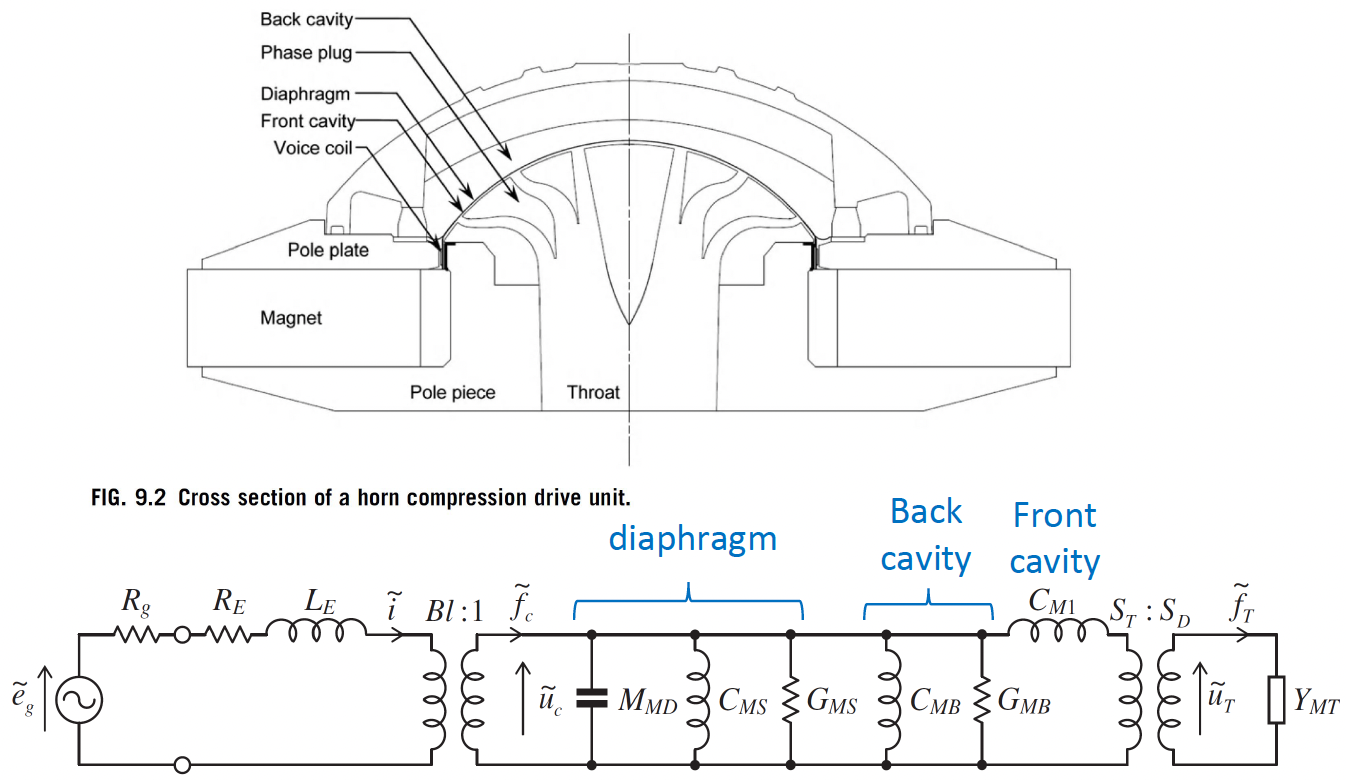
\includegraphics[width=0.90\textwidth]{horn_circuit.png}
    \caption{Electro-mechano-acoustical equivalent circuit of the compression driver and horn (admittance analogy). The driver electrical branch (voice coil \(R_{EC}\), \(L_{EC}\)) drives the mechanical section (diaphragm mass \(M_{MD}\), compliance \(C_{MS}\), damping \(R_{MS}\)) through the transformer of ratio \(Bl\colon 1\). The mechano-acoustic transformer of ratio \(1\colon S_T\) delivers power to the horn throat admittance \(Y_{MT} = 1/(\rho_0 c S_T)\)}
\end{figure}

\section{Horn Profile and Acoustic Gain}
\label{sc:103}

\subsection{Exponential Horn and Cutoff Frequency}
\label{ssc:1031}

The most widely used horn profile is the exponential horn, in which the cross-sectional area expands as:
\[
S(x) = S_T e^{m x}
\]
where \(x\) is the axial coordinate measured from the throat and \(m\) is the flare constant (in \(\si{\per\meter}\)) that controls how rapidly the cross-section expands.
The exponential profile provides the best approximation to a constant-resistance acoustic transmission line: for frequencies above the cutoff frequency, the horn presents a nearly resistive input impedance to the driver.

The cutoff frequency of the exponential horn is:
\begin{equation}
    f_c = \frac{m c}{4\pi}
    \label{eq:hornCutoff}
\end{equation}
Below \(f_c\), the wave equation in the horn has no propagating solutions: acoustic energy is reflected back toward the throat and the horn no longer transmits sound efficiently.
A larger flare constant \(m\) produces a wider-flaring horn with a higher cutoff frequency; a smaller \(m\) produces a narrower horn with a lower cutoff.
Extending the bass response of a horn system requires either a lower \(m\) (gentler flare) or a larger mouth area, both of which increase the physical size of the horn.

\subsection{Alternative Horn Profiles}
\label{ssc:1032}

Several other cross-sectional profiles are used in practice, each offering a different trade-off between bandwidth, directivity, and physical size.

\begin{figure}[!htb]
    \centering
    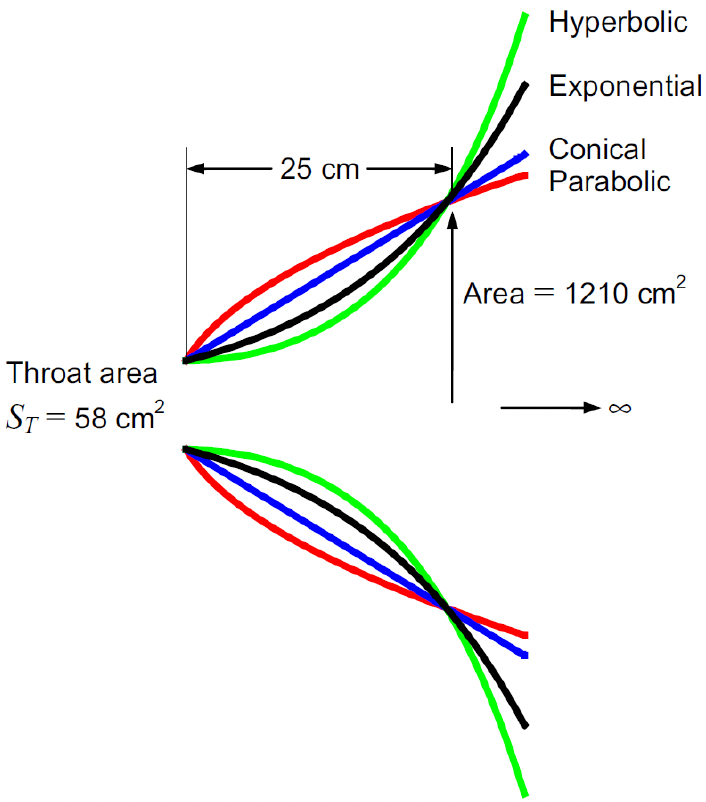
\includegraphics[width=0.60\linewidth]{horn_profiles.png}
    \caption{Cross-sectional profiles of four common horn geometries: exponential, conical, hyperbolic (hypex), and tractrix. The exponential profile provides smooth impedance matching; the tractrix minimizes internal reflections; the conical is simplest to manufacture; the hyperbolic allows independent control of mouth impedance and flare rate}
\end{figure}

The conical horn is the simplest to manufacture and analysis: the area grows as \(S(x) \propto x^2\) from a virtual apex.
It provides good directivity control but less efficient impedance matching than the exponential.
The hyperbolic (or hypex) profile allows the designer to independently control the throat impedance and the expansion rate, making it useful when both low-frequency extension and controlled directivity are required.
The tractrix profile is derived by requiring that wavefronts emerge from the mouth with minimum internal reflection; it is widely used in high-quality studio monitoring horns because its smooth flare minimizes the colorations introduced by reflections inside the horn.

\subsection{Radiation Impedance of the Horn Throat}
\label{ssc:1033}

The normalized throat impedance \(Z_T/(\rho_0 c S_T)\) of a horn depends on both the horn profile and the frequency, and it varies significantly among the different geometries.

\begin{figure}[!htb]
    \centering
    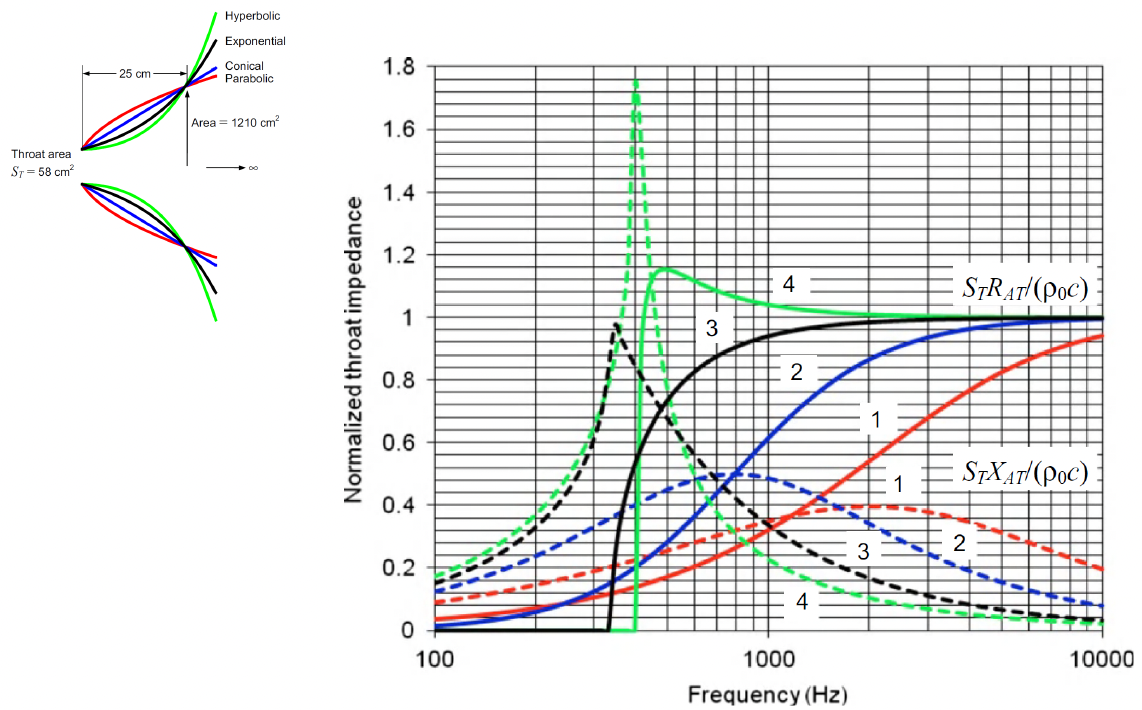
\includegraphics[width=0.65\linewidth]{horn_impedance.png}
    \caption{Normalized throat impedance for four horn profiles: infinite parabolic (1), conical (2), exponential (3), and hyperbolic (4). The resistive part (solid) determines the power transferred to the air; the reactive part (dashed) represents stored energy. Above the cutoff frequency, all profiles approach the plane-wave limit \(\mathrm{Re}[Z]/(\rho_0 c S_T) \to 1\)}
\end{figure}

For the exponential horn above cutoff, the real part of the normalized throat impedance rises steeply from zero at \(f_c\) to unity at high frequencies, confirming that the horn loads the driver with a nearly resistive impedance over its operating band.
Below cutoff, the real part collapses to zero and the throat impedance becomes purely reactive: the driver is loaded by a spring-like or mass-like reactance and no net power is transferred to the air.
This transition from resistive to reactive loading at \(f_c\) is the acoustic analogue of the cutoff of a waveguide, and it sets the hard lower limit of the horn's operating band.

\subsection{Acoustic Gain and Maximum Theoretical Sensitivity}
\label{ssc:1034}

The pressure transformation ratio of the horn from throat to mouth is set by the area ratio \(S_M/S_T\).
In the ideal lossless horn operating above cutoff, the acoustic pressure at the mouth is related to the pressure at the throat by:
\[
\frac{\tilde{P}_T}{\tilde{P}_M} = \sqrt{\frac{S_M}{S_T}}
\]
The maximum theoretical acoustic gain, measured as the ratio of the axial far-field SPL produced by the horn to that of the same driver operating as a direct radiator into free air, is:
\begin{equation}
    G_\mathrm{max} = 20\log_{10}\left(\frac{S_M}{S_T}\right) \quad [\mathrm{dB}]
    \label{eq:hornGain}
\end{equation}
A compression driver with a diaphragm area \(S_D = \pi (5 \mathrm{cm})^2 \approx \SI{78}{\centi\meter\squared}\) coupled through a throat of area \(S_T = \pi (1 \mathrm{cm})^2 \approx \SI{3}{\centi\meter\squared}\) achieves a theoretical gain of \(20\log_{10}(78/3) \approx \SI{28}{\decibel}\).
In practice, internal reflections, diffraction losses at the mouth, and non-ideal wavefront geometry reduce this by 5 dB to 10 dB, but even the achievable gain of 15 dB to 25 dB represents an enormous improvement in sensitivity compared to direct-radiating designs.

\subsection{Directivity and Bandwidth}
\label{ssc:1035}

The far-field directivity of a horn loudspeaker is controlled by the mouth geometry.
At low frequencies (mouth circumference much smaller than the wavelength), the radiation is nearly omnidirectional.
As frequency rises and the mouth dimensions become comparable to the wavelength, the radiation narrows into an increasingly sharp beam along the horn axis, following the same physics as the piston directivity analyzed in chapter \ref{ch:sound_radiation}.
The cutoff frequency at which the mouth starts to beam is:
\[
f_0 = \frac{c}{2\pi a_M}
\]
where \(a_M = \sqrt{S_M/\pi}\) is the equivalent radius of the mouth.
The table in chapter \ref{ch:sound_radiation} (section \ref{sc:62}) gives representative values: a mouth of radius \SI{30}{\centi\meter} has \(f_0 \approx \SI{183}{\hertz}\), so the horn is effectively omnidirectional below that frequency and progressively more directional above it.
Constant-directivity (CD) horn designs address the high-frequency beaming problem by modifying the flare shape near the throat to introduce controlled diffraction, maintaining a uniform coverage angle across the operating band at the cost of some efficiency.
These designs are standard in professional sound reinforcement, where consistent audience coverage is more important than maximum on-axis sensitivity.

\begin{figure}[!htb]
    \centering
    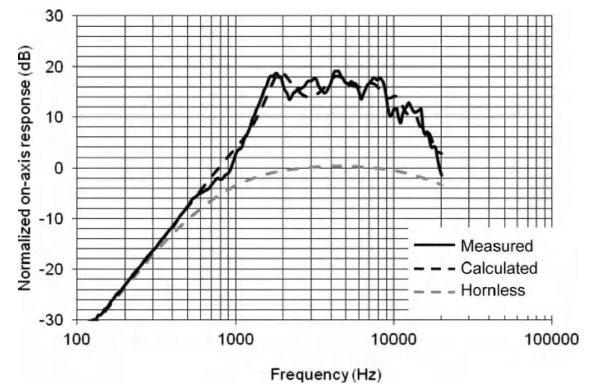
\includegraphics[width=0.55\linewidth]{horn_directivity.png}
    \caption{On-axis SPL frequency response of a high-frequency horn driver (solid curve). The flat response region extends from approximately \SI{1}{\kilo\hertz} to \SI{20}{\kilo\hertz}, corresponding to the band in which the horn presents a resistive throat impedance and the driver diaphragm operates in its mass-controlled regime}
\end{figure}
